\documentclass[11pt]{article}
\usepackage{url}
\usepackage{verbatim}
\usepackage{graphicx}
\usepackage{mathptmx}

\newcommand{\daj}{\textsc{DAJ}}
\newcommand{\p}[1]{\texttt{#1}}
\newcommand{\bu}[1]{\textsf{#1}}

\textwidth=15cm
\textheight=22cm	
\topmargin=0pt
\headheight=0pt
\oddsidemargin=1cm
\headsep=0pt
\renewcommand{\baselinestretch}{1.1}
\setlength{\parskip}{0.20\baselineskip plus 1pt minus 1pt}
\parindent=0pt

\title{\daj{} - Distributed Algorithms in Java\\User's Guide\\\mbox{}\\\large{Version 3.5}}
\author{Mordechai (Moti) Ben-Ari\\
Department of Science Teaching\\
Weizmann Institute of Science\\
Rehovot 76100 Israel\\
\textsf{moti.ben.ari@gmail.com}\\
\url{https://www.weizmann.ac.il/sci-tea/benari/home}}
\date{18 January 2006\\\smallskip
Modernized 7 October 2020}
\begin{document}

\maketitle
\thispagestyle{empty}

\vfil

\begin{center}
Copyright (c) 2003--2006, 2020 by Mordechai (Moti) Ben-Ari.
\end{center}
Permission is granted to copy, distribute and/or modify this document
under the terms of the GNU Free Documentation License, Version 1.2
or any later version published by the Free Software Foundation;
with Invariant Section ``Introduction,'' no Front-Cover Texts, and no Back-Cover Texts.
A copy of the license is included in the file \p{fdl.txt}
included in this archive.
\vfil
\newpage

\section{Introduction}

\daj{} is an interactive, visual aid for studying distributed
algorithms. \emph{Interactive}, because you must explicitly
specify every step of the execution sequence.
\emph{Visual}, because the state of the nodes is continuously
displayed. \emph{Study aid}, because they solve one of the most
difficult problems encountered by students of these algorithms
by automatically doing the necessary ``book-keeping.'' The
program can create a log file of commands so that you can
automatically replay scenarios until you understand them. You can implement other algorithms with an elementary knowledge of Java.
Visualizations are included for the virtual global structures
constructed by some of the algorithms.

The following algorithms are implemented:
\begin{enumerate}
\item Berman-Garay (King) algorithm for consensus
\item Byzantine generals algorithm for consensus (byzantine failures)
\item Byzantine generals algorithm for consensus (crash failures)
\item Chandy-Lamport algorithm for global snapshots
\item Dijkstra-Scholten termination detection
\item Flooding algorithm for consensus
\item Lamport algorithm for mutual exclusion
\item Ricart-Agrawala algorithm for mutual exclusion
\item Maekawa mutual algorithm for exclusion
\item Suzuki-Kasami algorithm for mutual exclusion
\item Huang credit-recovery termination detection
\item Mattern credit-recovery termination detection
\item Carvalho-Roucairol token algorithm for mutual exclusion
\item Neilsen-Mizuno algorithm for mutual exclusion
\end{enumerate}



\subsection{Acknowledgments}
I wish to thank Judith Bishop of the University of Pretoria for
her pioneering use of this software in her classes. University
of Pretoria students Richard McGladdery, Frederick Kemp, Frank
Harvie, Derick Burger, Darrell Newing and Leoni Lubbinge wrote
several of the algorithms, which were adapted to version 2 by
Basil Worrall. Basil also found some bugs in version 3. The
virtual trees for the Byzantine Generals algorithm were designed
by Ahuva Tikvati of the Weizmann Institute of Science and
programmed by Antoine Pineau of the University of Joensuu. The
visualization of the spanning tree of the Dijkstra-Scholten
algorithm is based upon a program by Maor Zamsky.
Otto Sepp\"al\"a and Ville Karavirta of the Helsinki University
of Technology implemented the credit-recovery and token-passing
algorithms.

\subsection{References} \daj{} was first described in Distributed
Algorithms in Java. \emph{ACM SIGCSE Bulletin} 29(3), 1997, 62-64.
A revised version was published as: Interactive Execution of
Distributed Algorithms. \emph{ACM Journal of Educational
Resources in Computing} 1(2), 2001.

The graphics display of the BG algorithm is described in:
Ahuva Tikvati, Mordechai Ben-Ari, Yifat Ben-David Kolikant.
Virtual trees for the Byzantine Generals algorithm
\textit{Thirty-Fifth SIGCSE Technical Symposium on Computer Science Education}.
Norfolk, VA, 2004. Also published in \textit{ACM SIGCSE Bulletin} 36(1), 2004.

\subsection{Download}

\daj{} can be downloaded from \url{https://github.com/motib/daj}.

\section{Installation}

Download the \daj{} distribution file called \p{dajN.zip},
where \p{N} is the version number.
Open the file into a clean directory, preferably \verb=\=\p{daj}.
This will create subdirectories \p{docs} for the documentation,
\p{daj} for the source files and
\p{meta-inf} for the Java manifest file.

To rebuild \daj{}, execute \p{build.bat}, which will create the
file \p{daj.jar}.

\section{Running \daj{}}\label{s.run}

\subsection{Executing the program}

Execute \p{run.bat} which contains the command \p{java -jar daj.jar \%1 \%2}.
The two optional parameters are the algorithm code and the number of nodes. Execute \p{run help} to obtain a list of the codes. Alternatively, the algorithm and number of nodes can be chosen interatively from the menu that appears when \daj{} is started.

\subsection{Description of the display}
The structure of the display for each algorithm is identical (Figure~\ref{fig1}).
At the bottom of the screen is a line containing buttons that globally affect
all the nodes.
Most of the screen is devoted to a grid of panels, one for each node.
Each node panel contains a pair of lines for the data of the node, followed
by a pair of lines for each of the other nodes.
At the bottom of each node panel is a line of buttons for choosing a step
of the algorithm. The contents of these buttons change according to the
state of the node.
The data for each node is color-coded.

\begin{figure}[t]
\begin{center}
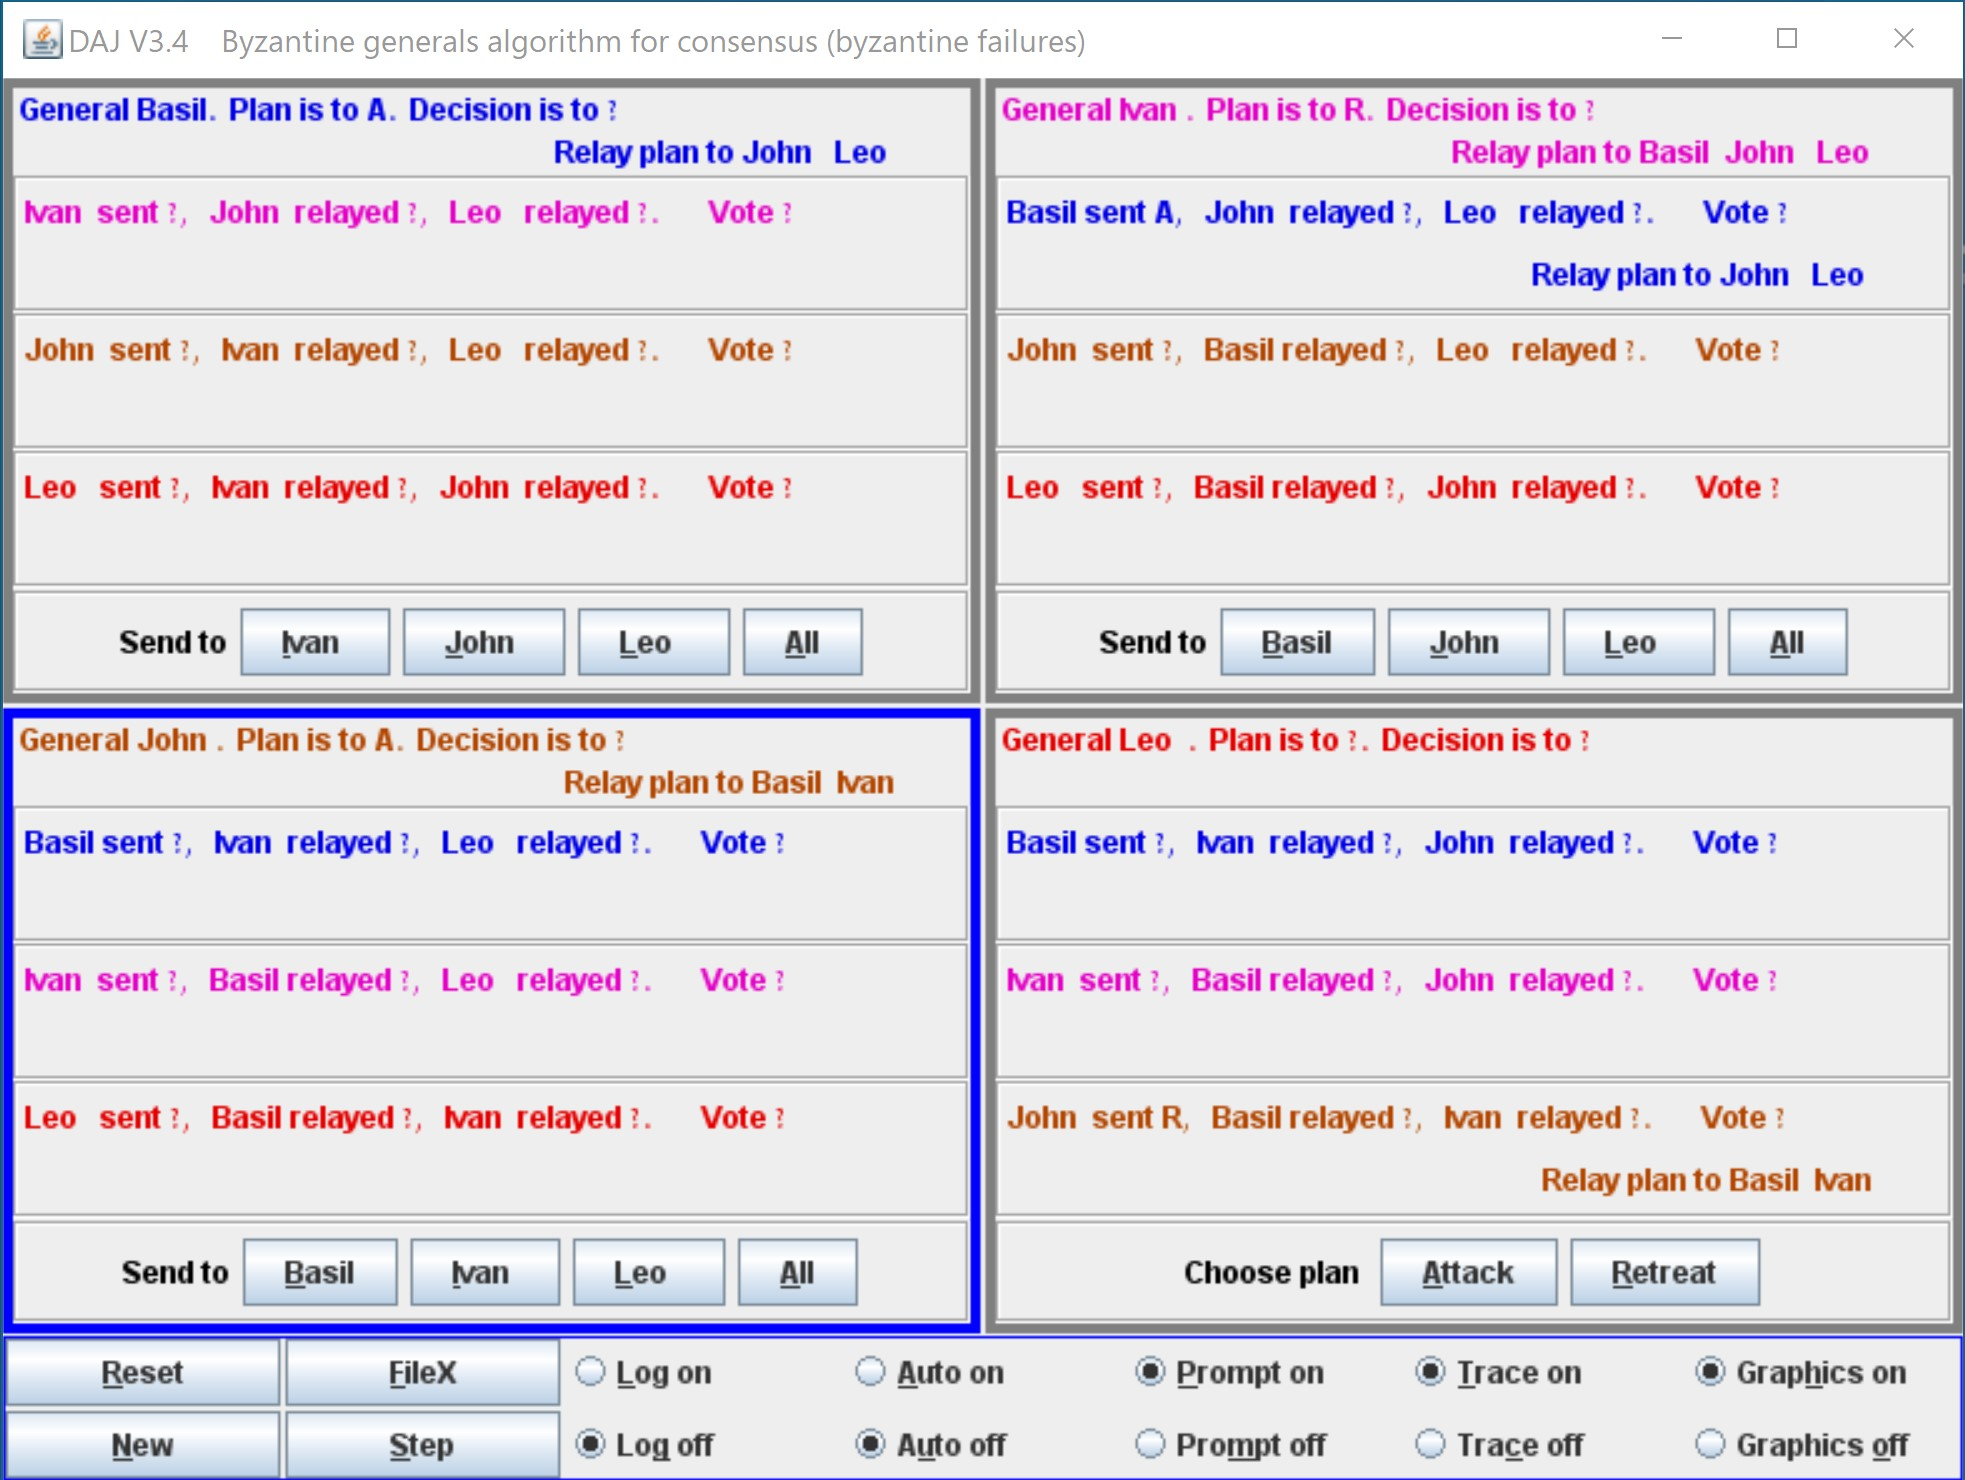
\includegraphics[width=15cm,keepaspectratio=true]{daj.jpg}
\end{center}
\caption{The algorithm window}\label{fig1}
\end{figure}

\begin{figure}[htb]
\begin{center}
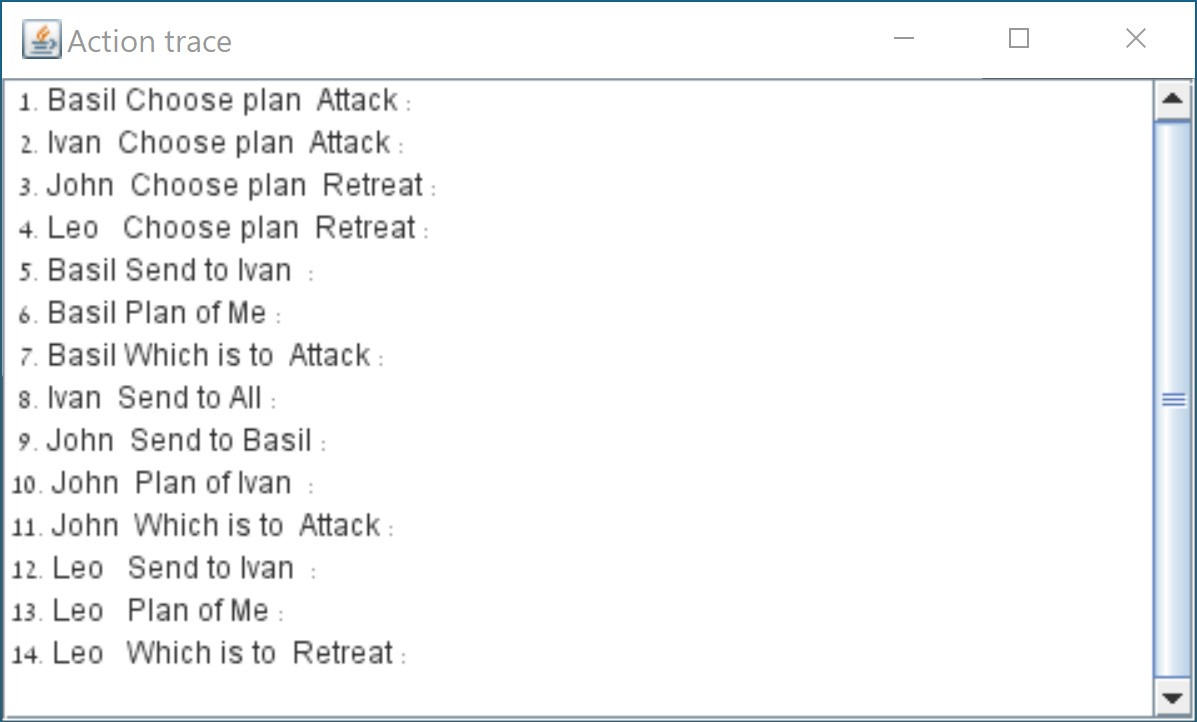
\includegraphics[width=10cm,keepaspectratio=true]{trace.jpg}
\end{center}
\caption{The action trace}\label{fig2}
\end{figure}

\subsection{Creating a scenario}
%\begin{itemize}
To perform a step of the algorithm, select a button in one of the nodes.
The data structure is updated and the action is written on the log file
and in the action trace window (Figure~\ref{fig2}).
Some buttons may not be active. It is a test of your understanding of the
algorithm that you not click on a non-active node, though if you do so,
the data structure is not changed. The reason that the node is not active
is written on the log file and
in the action trace window.\footnote{This feature is currently implemented
only for the Ricart-Agrawala
and Byzantine Generals algorithms.}
The second line of each pair in each node are prompts to remind you what messages to send.
The \p{All} button enables you to send multiple messages such as requests
or replies to all other nodes.
%\end{itemize}

\newpage

\subsection{Algorithm-independent buttons}
\begin{description}
\item[\p{Reset}] Return all the nodes to their initial state.
\item[\p{New}] Terminate the execution of the algorithm and return
to algorithm selection menu. To terminate execution of the program,
close the window or select \p{New} and then \p{Exit}.
\item [\p{FileX}, \p{ Step}, \p{ Log on/off}, \p{ Auto on/off}]
Buttons for working with the log file (Section~\ref{s.log}).
\item[\p{Prompt on/off}] Toggles display of the prompt lines.
Normally, prompts will be on initially and can be turned off for assessment.
\item[\p{Trace on/off}] Toggles display of the action trace window.
Normally, it will be on initially and can be turned off for assessment.
\item[\p{Graphics on/off}] Toggles display of the graphics window.
Currently, this is implemented only for displaying virtual trees for the
Byzantine Generals algorithm, the spanning tree for the Dijkstra-Scholten
algorithm and the implicit queue for the Ricart-Agrawala algorithm.
\end{description}

\subsection{Using the keyboard}
Each button has a mnemonic. If you press \p{Alt-Key},
the \p{Key} is directed to the global button line at the button, e.g.
\p{Alt-r} will cause a reset.
Otherwise, the key is directed to the ``current'' node
which is indicated by the colored border. The \p{Enter} key cycles
through the nodes; clicking with the mouse will also cause that node to
become the current one.

\subsection{Writing and reading a log file}\label{s.log}
Actions are written to the file \p{logout.txt} as ordinary character strings:
the number of the node and the text of the button,
followed if needed by a comment for the reason that
the selection has been rejected.
You can rerun a scenario from the file \p{login.txt} by selecting \p{Auto on}.
To execute, click on \p{Step}.
When end of file is reached, \p{Auto off} is set and you can continue issuing commands manually.
If you \p{Reset} the algorithm, both \p{login.txt} and \p{logout.txt} are reset
to the beginning.
Selecting \p{FileX} will cause a file exchange:
\p{login.txt} will be deleted and \p{logout.txt} will be renamed as \p{login.txt}.
This command enables you to create a scenario, and then rerun it one or more times without
leaving the program.
You can always edit, save or rename these files outside the program.

\section{Using \daj{} in the classroom}
\daj{} can be used with a screen projector
to demonstrate scenarios of an algorithm.
In the lab, you can require the students to create one or more
scenarios that correctly follow the algorithm from start to finish.
This is a non-trivial task and will help the student develop
a full understanding of the algorithm.
For further lab work or homework, pose questions that can
be solved by creating and analyzing scenarios.
The following example (adapted from an examination question
written by Yifat Ben-David Kolikant) shows how scenario-based
questions can be posed.

In the algorithm for the Byzantine Generals, suppose that
there is exactly one traitor and that the panel for Zoe displays
the following information:
\begin{verbatim}
   General Zoe . Plan is A. Decision is to XX.
   John  sent A, Leo  relayed A, Basil relayed R.   Vote XX.
   Leo   sent R, John relayed R, Basil relayed R.   Vote XX.
   Basil sent R, John relayed A, Leo   relayed R.   Vote XX.
\end{verbatim}
\textbf{Question:} Can you tell who the traitor is?
\textbf{Answer:} You cannot tell who the traitor is, but you can tell that
it isn't Leo. Since there is only one traitor, John and Basil
must both be loyal. But then they can't disagree on what John
thinks: John sent A while Basil relayed R.

\textbf{Question:} Fill in the
values marked XX. \textbf{Answer:} The preliminary votes are A, R, R
(from top to bottom). Together with Zoe's plan of A, the final
vote is 2--2, and ties are resolved in favor of R.

\textbf{Question:} Create
a scenario leading to this display for Zoe. Use the minimum
number of steps to obtain this display. \textbf{Answer:} Let John be the
traitor. Leo and Basil who are loyal both choose Retreat and
relay their plan truthfully. John sends Retreat to Leo, and
Attack to both Zoe and Basil.

\textbf{Question:} What is displayed for the
other generals? \textbf{Answer:} Here is the display after a minimal
scenario with John as the traitor.

\begin{verbatim}
   General Zoe . Plan is A. Decision is to R
                          Relay plan to John Leo Basil
   John  sent A, Leo  relayed A, Basil relayed R.   Vote A
                          Relay plan to Leo Basil
   Leo   sent R, John relayed R, Basil relayed R.   Vote R
                          Relay plan to John Basil
   Basil sent R, John relayed A, Leo   relayed R.   Vote R
                          Relay plan to John Leo

   General John . Plan is A. Decision is to ?.
   Zoe   sent ?, Leo  relayed ?, Basil relayed ?.   Vote ?.
   Leo   sent R, Zoe  relayed ?, Basil relayed ?.   Vote ?.
                          Relay plan to Basil
   Basil sent R, Zoe  relayed ?, Leo   relayed ?.   Vote ?.
                          Relay plan to Leo

   General Leo  . Plan is R. Decision is to ?.
   John  sent A, Leo  relayed ?, Basil relayed ?.   Vote ?.
                          Relay plan to Basil
   Zoe   sent ?, John relayed ?, Basil relayed ?.   Vote ?.
   Basil sent R, John relayed ?, Zoe   relayed ?.   Vote ?.
                          Relay plan to John

   General Basil. Plan is R. Decision is to ?.
   John  sent R, Leo  relayed ?, Basil relayed ?.   Vote ?.
                          Relay plan to Leo
   Zoe   sent ?, Zoe  relayed ?, Basil relayed ?.   Vote ?.
   Leo   sent R, Zoe  relayed ?, Leo   relayed ?.   Vote ?.
                          Relay plan to John
\end{verbatim}

\section{Algorithm-specific actions}

\subsection{Byzantine Generals}
L. Lamport, R. Shostak, M. Pease.
The Byzantine generals problem.
\emph{ACM Transactions on Programming Languages and Systems}
4(3), 1982, 382-401.

This famous algorithm is used to demonstrate the implementation
of a reliable system in the presence of faults. A loyal general
will relay messages exactly as they are received, while a
traitorous general may relay a message incorrectly. The goal of
the algorithm is for the loyal generals to come to a consensus
in the presence of traitors. Three loyal generals can come to a
consensus even in the presence of a fourth general who is a
traitor.

First, select attack or retreat for each general. Next, relay the
chosen plans to each of the other three generals. While this is
being done, you may receive the plan of another general; these
plans must eventually be relayed to the remaining two generals.

The \p{All} button sends or relays the correct data
to the other nodes as would be done by a loyal general. For a
traitor, you must send messages one by one.

A two-stage majority voting scheme is used. Majority voting (2
out of 3) is used by each general to decide what the true plan
of the other generals is. The presence of a single traitor does
not affect the outcome of this vote, so each loyal general has
an identical picture of the plans chosen by the other two loyal
generals. A second stage of majority voting is used to decide
what plan to follow.

The program does not maintain information as to who is a traitor
and who is not. You must specify state transitions that are
consistent with the algorithm. The applet does keep track of
which plans have been sent and received, and the prompt lists
will tell you which plans must be sent or relayed. Voting is
done automatically.

\subsection{Virtual trees for the Byzantine Generals Algorithm\\
with Ahuva Tikvati and Antoine Pineau}

The program dynamically constructs \emph{knowledge trees} for each general (Figure~\ref{fig3}).
A knowledge tree is a data structure
containing the global knowledge \emph{about} the plan of a
general, not the data structure contained locally at each node.
The root of the tree contains the general's selection (attack or
retreat). For each message sent, a node is created for the
recipient of the message. If the sender is a traitor (sending
the plan opposite the one received), the traitorous message
labels the outgoing edge. These trees are helpful for
understanding how the two-stage voting is performed and hence
why the algorithm is correct.

\begin{figure}[htb]
\begin{center}
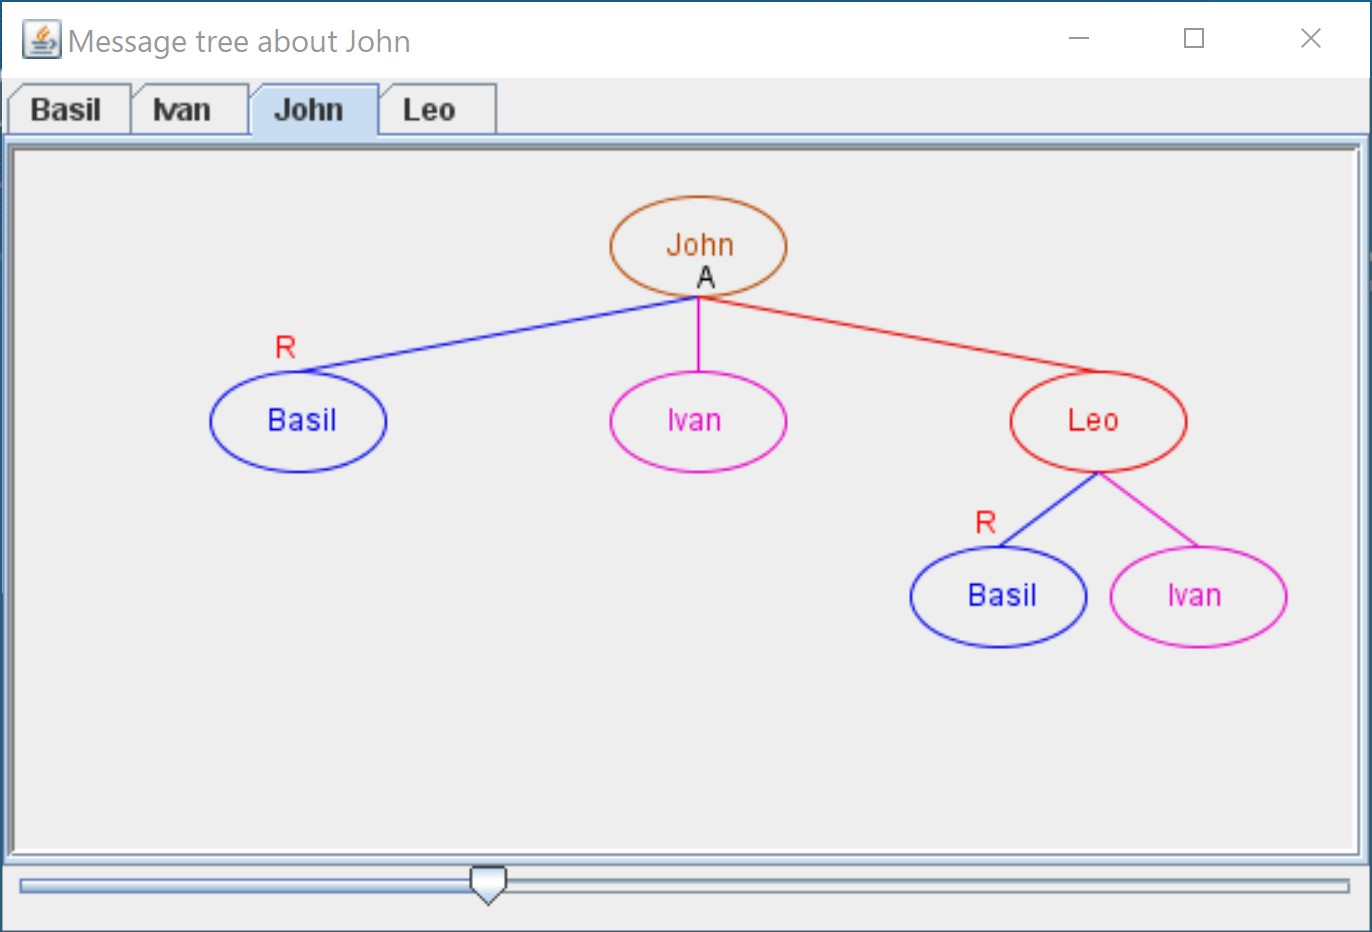
\includegraphics[width=10cm,keepaspectratio=true]{tree.jpg}
\end{center}
\caption{The virtual trees}\label{fig3}
\end{figure}

The root of the tree for general G is labeled with the name
of the general and the plan that he chose.
When another general G' receives the plan of G directly from G,
a child node is created created for G' and labeled with his name.
If G' then relays the plan of G to another general G'',
a child node of G' for G'' is similarly created.
If a general correctly transmits the original or received plan,
the edge to that son is not labeled;
however, if the message is sent by a traitor, the edge is labeled with its contents.
You can select the panel corresponding to the
knowledge tree of general G by clicking on tab labeled G.
The width of the tree can be changed using the slider.

\subsection{Crash Failure}

This algorithm is adapted from the EIGStop algorithm in Section 6.2.3 of
Nancy Lynch. \emph{Distributed Algorithms}. Morgan Kaufman, 1996.

This is a simpler version of the Byzantine Generals algorithm.
Nodes are only allowed to \emph{crash}, that is, to stop sending
messages; they are not allowed to send an incorrect message.
Other nodes know that the node has crashed (perhaps using a
timeout). The number of nodes is not significant for the
correctness of the algorithm.

The operation is the same as for BG, except that once a node has
selected \p{Crash}, it must continue to reply \p{Crash} to each
outstanding message.

\subsection{Dijkstra-Scholten Termination}

E.W. Dijkstra, C.S. Scholten.
Termination detection for diffusing computations.
\emph{Information Processing Letters} 11(1), 1980, 1-4.

A set of nodes is made to terminate by creating an implicit
spanning tree. The source node that is the root of the spanning
tree is compiled-in. When you send messages, the first one
received by a node defines its parent in the tree.
The virtual spanning tree is displayed in the visualization frame.

For each message received, you must eventually send a signal on
the back channel. When you select terminate for a node, you must
``cover'' the deficits (messages less signals) on all the
incoming edges (except for that from its parent node) by sending
signals. When signals have been received from each outgoing
edges so that its outgoing deficit returns to zero, you can send
the last signal to its parent node.
The program keeps track of deficits and prevents sending the
final signal until the outgoing deficit is zero.

% Otto: Changed the description.
\subsection{Huang Termination Detection
by Richard McGladdery, Frederick Kemp and Otto Sepp\"al\"a}

Huang S.-T.
Detecting termination of distributed computation by external agents.
\emph{Proceedings IEEE 9th International Conference on
Distributed Computing Systems},
1989, 79-84.

\emph{Implementation in DAJ by Otto Sepp\"al\"a, Helsinki University of Technology}.

In the sense of Huang's algorithm a distributed computation consists of
a set of processes which communicate with each other by message passing.
Each process can either be either \emph{active} or \emph{idle}.
An active process may become idle at any time.
An idle process can become active on receiving a \emph{computation}
message. Computation messages are those that are related to the underlying
computation being performed by the cooperating processes. A computation
is said to have terminated if and only if all the processes are idle and
there are no messages in transit. The messages sent by the termination
detection algorithm are referred to as \emph{control} messages.

One of the cooperating processes monitors the computation
and is called the \emph{controlling agent}.
Initially all processes are
idle, the controlling agent's weight equals 1, and the rest of the processes
is zero. The computation starts when the controlling agent sends a computation
message to one of the processes. Any time a process sends a message, the
process's weight is split between itself and the process receiving the
message (the message carries the weight for the receiving process). The
algorithm therefore assigns a weight $W (0 < W <= 1)$ to each active
process (including the controlling agent) and to each message in transit.
The weights assigned are such that, at any time, they satisfy an invariant
$W = 1$. On finishing the computation,
a process sends its weight to the controlling agent, which adds the received
weight to its own weight. When the weight of the controlling agent is once
again equal to 1, it concludes that the computation has terminated.

If floating point numbers were used to represent weights, we would soon run
into problems with rounding errors. To overcome this, Huang describes a
modified floating point scheme, where the controlling agent holds a massive
fixed point number that holds all the weight not distributed in the system.
The fixed point number is divided to smaller parts, slots, each of which can be
thought of as a small floating point number. The slot number is the exponent
and the bits inside the slot the mantissa.

Each process holds one such floating point number. The arithmetic works as
for floating point numbers. Splitting is done with the mantissa as long as possible,
until we must change the exponent. The reverse applies to addition.
The fact that the controlling agent has the whole
fixed point number solves the floating point calculation problems. When two
weights with different slot numbers (exponents) are being added, the smaller
of the two is sent to the controlling agent which can always add it to the
fixed point number.

If a process ever reaches the maximum slot number it might not be able to split
its weight. In this case it can make a supply request to the controlling agent
for more weight, which will send the supply as any is or becomes available.
If the process terminates before receiving the supply, it sends the supply
back to the controlling agent.

An example of a scenario can be found in the file \bu{hgexample.html}.

\subsection{Mattern Global Quiescence Detection Algorithm}

Mattern F.
Global quiescence detection based on credit distribution and recovery.
\emph{Information Processing Letters}, Volume 30, Number 4, p. 195-200, 1989.

\emph{Implementation in DAJ by Otto Sepp\"al\"a, Helsinki University of Technology}.

The Mattern algorithm is essentially the same algorithm as Huang's algorithm.
One difference is in the implementation of the weights (here credits). While
Huang allowed for a mantissa (slot size) of a desired size, Mattern only deals
with the exponents. The other difference is that the controlling agent (called
environment in this algorithm) counts the credit debt distributed in the system
(not the remaining weight as in Huang). The debt is saved as a set of exponents.

Splitting a weight is equal to changing one exponent into two that are both
one bigger than the original. Again all the other rules are just basic binary addition
and subtraction rules.

\subsection{Flooding algorithm for consensus with crashing}

Based upon Section 6.2 of Nancy Lynch. \emph{Distributed Algorithms}. Morgan Kaufman, 1996.

\subsection{Byzantine Generals with King}

This algorithm is due to Berman and Garay, Cloture votes: n/4-resilient
distributed consensus in t+1 rounds. \emph{Mathematical Systems Theory}
26, 1(1993), 3-19.
It was taken from Algorithm 5.2 of Hagit Attiya and Jennifer Welch.
\emph{Distributed Computing}. McGraw-Hill, 1998.


Compared with the original BG algorithm,
for one traitor, you need four (rather than three) loyal generals,
and four (rather than two) rounds of message passing.
The advantage is that the number of messages is constant even if
the number of traitors increases,
whereas in the BG algorithm, the number of messages increases
exponentially.

The program has the number of traitors compiled in as 1,
and the first king selected as node 0, with the kingship
passed in cyclic numerical order.

After receiving a round of messages, each node computes a
majority decision \emph{and} the number of votes that the
majority received. Then there is a second round of messages,
where one node is specified to be the king who sends his
majority decision to the other nodes. A receiving node changes
its own plan to that of the king \emph{unless} the majority
decision was decided by an \emph{overwhelming} majority (defined
as more than n/2 + number of traitors), in which case it adopts
the majority decision. A second pair of rounds is now conducted,
with a different king.

Assuming only one traitor: either the first king is loyal or the
second king is loyal. If the first, the other loyal generals
will adopt his plan; if the second, after the loyal generals
adopt his plan on the first pair of rounds, the majority during
the second pair will be overwhelming, and the traitor will not
be able to overturn it.

Operations: after sending all messages of the first round, the
majorities are computed. Then, only the king can send messages
while the others wait. After the first pair of rounds, the state
machine is paused so that you can check the data. Click
\p{Continue} to commence the second pair of rounds.
\subsection{Lamport mutual exclusion by Leoni Lubbinge}

L. Lamport. Time, clocks, and the ordering of
events in a distributed system.
\emph{Communications of the ACM} 21(7), 1978, 558-565.

Every site Si keeps a queue, \p{request\_queuei}, which contains mutual exclusion
requests ordered by their timestamps.

\textbf{Requesting the critical section:}
When a site Si wants to enter the CS, it sends a \p{request(tsi,i)} message
to all sites in its request set and places the request on \p{request\_queuei}.
When a sites Sj receives the \p{request(tsi,i)} message from Si, it return
a timestamped \p{reply} message to Si and places Si's request on \p{request\_queuej}.

\textbf{Executing the critical section:}
Site Si enters the CS when the following conditions hold.
Si has a received a message with timestamp larger than (tsi,i) from all
other sites.
Si's requests is at the top of \p{request\_queuei}.

\textbf{Releasing the critical section:}
Site Si, upon exiting the CS, removes its request from the top of its request
queue and sends a timestamped \p{release} message to all sites in its request set.
When a site Sj receives a \p{release} message from site Si, it removes Si's
request from its request queue.

When a site removes a request from its request queue, its own request may
come at the top of the queue, enabling it to enter the CS. The algorithm
executes CS requests in the increasing order of timestamps.

To minimize the number of messages send and improve performance,
the following changes were made:
If site Sj receives a \p{request} message from Si after it has sent its own
\p{request} message with timestamp lower than the timestamp of Si's request,
it doesn't send a \p{reply} message.
If site Sj receives a \p{request} message from Si while it is busy executing
the CS, it doesn't send a \p{reply} message.
If a site Si receives a \p{release} message from a site Sj while it is waiting
for a \p{reply} message from site Sj, it treats the \p{release} message as a \p{reply}
message as well.

To disambiguate the case where two sites request the CS simultaneously,
the following change was made:
If two sites Si and Sj sends out \p{request} messages with the same timestamp,
the site with the highest site number is put on the request queue before
the other site.

\subsection{Maekawa mutual exclusion by Derick Burger and Darrell Newing}

Maekawa Mamoru.
A $\sqrt{N}$ algorithm for mutual exclusion in
decentralized systems.
\emph{ACM Transactions on Computer Systems}, 3(2), 1985, 145-159.

This algorithm achieves mutual exclusion by maintaining a subset
of the sites participating in the algorithm. A site has to send \p{request}
messages to all the sites in this request set(R). When a site in this
request set receives a \p{request} message, it sends back a \p{reply} message
to the sender. If it has already sent a \p{reply} message to someone else,
it simply queues up the \p{request} so that it can be replied to later.
Note that Maekawa's queue is only a single site queue. Once the sending
site has received all the \p{reply}'s from the request set sites, it may
enter the critical section. Release of the critical section is similarly
handled with \p{release} messages.

Example 1:
Select \p{Enter Critical Section} for John
Send a \p{Request} to all John's neighbors.
For each participant, select \p{Reply} to send a reply to John.
John can now enter the critical section. Select \p{Enter}.
John is now in the critical section.

Example 2, Deadlock demonstration:
Select \p{Enter Critical Section} for John.
Send a \p{Request} to all John's neighbors.
Select \p{Enter Critical Section} for Zoe, John and Zoe are now competing for the CS.
Send a \p{Request} to all Zoe's neighbors.
Send a \p{Reply} from Basil to John.
DEADLOCK ! Since one reply has already been sent out for one participant.

\subsection{Ricart-Agrawala Mutual Exclusion}

G. Ricart, A.K. Agrawala.
An optimal algorithm for mutual exclusion
in computer networks.
\emph{Communications of the ACM} 24(1), 1981, 9-17.

This is a generalized bakery algorithm for mutual exclusion.
Click \p{Choose} to choose a ticket number that is one greater
than the highest number received so far.
When a node has received a request, you must send a reply message
if the ticket number of the node is higher than the number in
the request or if the node does not want to enter its critical
section. Otherwise, the reply will be listed as deferred, and
you must send it only after the node has completed its critical
section.
This program checks the correctness of your sequence of steps: it
ensures that you choose a ticket number that is large enough,
and it keeps track of which replies need be made and which are
to be deferred.

The algorithm builds a virtual queue of all processes trying to enter their
critical section.
The queue is displayed in the visualization frame.
A node is added to the queue when the first request message from it is received
at another node and is removed from the queue when it leaves the critical section.


\subsection{Carvalho-Roucairol Mutual Exclusion}

O.S.F. Carvalho and G. Roucairol.
On mutual exclusion in computer networks.
\emph{Communications of the ACM} 26(2), 1983, 146-147.

\emph{Implementation in DAJ by Otto Sepp\"al\"a, Helsinki University of Technology.}

In the Ricart-Agrawala algorithm each entry to a critical section requires
$2*(N-1)$ messages to be sent. \emph{(Requests and replies to and from each node)}
Carvalho and Roucairol present a modification to the Ricart-Agrawala algorithm,
which reduces the required number of messages $2*(N-1)$ to just being an upper limit.

To enter its critical section, a node needs authorizations from all the other
nodes in the network. Information on authorizations over the
other nodes in the network is held in each node in an array
with one bit for each other node.

The essential idea behind this algorithm is that a node
trying to enter its critical section does not need to renew its authorization
from nodes it knows are not trying to enter their critical sections --- such nodes
do not send request messages. When attempting to enter the critical section,
a node does not have to send requests to any nodes it already holds the
authority over. This is where the savings from the messages are made.
 
As with the Ricart-Agrawala algorithm, the process with a higher ticket number
will yield to the a process that sent a request with a lower number by sending
a reply. A received reply gives the receiver the authorization over that node,
{\bf until that same node makes a request} at which point the authorization is lost.
If a request is received while in the critical section, the reply is deferred
and when the process exits the critical section, authorities held over such
nodes are immediately released.

\subsection{Suzuki-Kasami broadcast}

Suzuki Ichiro and Kasami Tadao.
A distributed mutual exclusion algorithm.
\emph{ACM Transactions on Computer Systems}, 3(4), 1985, 344-349.

\emph{Implementation in DAJ by Frank Harvie, University of Pretoria.}


If a site attempting to enter the critical section(CS) does not have
the token, it broadcast a \p{request} message for the token to all other sites.
A site that possesses
the token sends it to the requesting site upon receiving its \p{request}
message. If a site receives the \p{request} message while it is in the CS,
it sends the token only
after it has exited the CS. A site holding the token can enter its
CS repeatedly until it sends the token to some other site.

Example:
Select \p{Enter CS} for John
Select \p{Request CS} for Zoe and send requests to all Zoe's neighbours.
Zoe is now waiting for the Token.
Select \p{Request CS} for Basil and send requests to all his neighbours.
Basil is also waiting for the Token.
Select \p{Now} for John and Send the Token.
Select \p{Now} for Zoe and Send the Token.
Select \p{Now} for Basil.
John wants the CS, so select \p{Request CS} for him and request the token
from all of his neighbors.
John will be in the CS, select \p{Now} for him to exit the CS.

\subsection{Chandy-Lamport Snapshots}

K.M. Chandy, L. Lamport.
Distributed snapshots: Determining global
states of distributed systems.
\emph{ACM Transactions on Computer Systems} 3(1), 1985, 63-75.

The problem is to take a global snapshot of the state of a
distributed system, in particular, to account for messages that
may be within a channel.

To run the program, send and get an arbitrary number of messages,
and at some point, choose record from one or more nodes. Then
you must send markers to divide messages that have been received
from those still in the channel. Upon termination of the
snapshot, each message that has been sent is accounted for:
either it has been received or it is listed as having been in
transit.

% Ville: Added the description.
\subsection{Neilsen-Mizuno Algorithm for Mutual Exclusion}
M.L. Neilsen, M Mizuno.
A Dag-Based Algorithm for Distributed Mutual Exclusion.
\emph{11th International Conference on Distributed Computing Systems}, 1991, 354-360.

The Neilsen-Mizuno algorithm for distributed mutual exclusion is based
upon passing a token in a set of virtual trees constructed by the
algorithm.

A node that is the root and holds the token can enter its
critical section. Other nodes send requests to their immediate
parents. A node receiving a request can take one of the following actions.

\begin{itemize}
\item If the node is not the root of a virtual tree, the request is
relayed by the receiving node to its parent.
\item If the node is the root, it has the token, and it is not in the
critical section, it sends the token to the node that requested the
token.
\item If the node is the root and it is the critical section or
waiting for the token, it defers the request.
\end{itemize}

After exiting the critical section, the node sends the token to a
deferred node, if such exists.

In the implementation, the user can send the requests and receive the
messages. The messages are received when the user takes the required
action, thus the order of message arrival can be changed. For a
received request, the user can relay it to the parent, defer the node,
or send the token. However, only the correct action is allowed.

\section{Software structure}
The classes of \daj{} in the package \p{daj} are:

\p{daj.java} - The main program.

\p{AlgList.java} - Maintains the list of class, titles and
command-line parameters for each algorithm. It contains an inner
class \p{Interactive} which is a \p{JFrame} for selecting the
algorithm and the number of nodes.

\p{WaitObject.java} - A monitor type used for synchronization
between listeners and frames.

\p{Screen.java} - Builds the frame for the nodes, constructs the
global button panel, allocates instances of the algorithms and
allocates the logfile. It is the \p{ActionListener} for global
buttons, and the \p{KeyListener} for the entire program. The
following constants are public:

\begin{verbatim}
    String[] node          - the names  of the nodes.
    Color[]  color         - the colors of the nodes.
    Color    LABELCOLOR    - the color of the lables and buttons.
    boolean  isApplication - application or applet?
\end{verbatim}

\p{LogFile.java} - Opens, closes and renames files. Performs file
IO through a \p{BufferedReader}, \p{BufferedWriter} and
\p{StreamTokenizer}. Accessors \p{getNumToken} and
\p{getStringToken} return the integer and string parts of the
current command. Lookahead is done so the next command can be
displayed. \p{Screen} calls \p{step} when the button is pressed;
\p{LogFile} calls \p{doAction} of the node with the command.
When logging, \p{DistAlg} calls \p{write}.

\p{DistAlg.java} - This is an abstract class from which the
classes for the specific algorithms is derived. It encapsulates
all the awt/swing processing, so that the algorithms need only
work in terms of integers and strings. Derived classes must
implement the following abstract classes.

\begin{verbatim}
   abstract protected void init();
   // Algorithm-specific initialization.
   abstract protected int constructButtons();
   // Construct the button panels.
   //   Calls addComponents for each button panel
   //   and returns the initial button panel.
   abstract protected String constructTitle1();
   abstract protected String constructTitle2();
   abstract protected String constructRow1(int row);
   abstract protected String constructRow2(int row);
   // Construct the text for the two title lines
   //   and the two lines for each row.
   abstract protected boolean stateMachine(String command);
   // Implement the state machine.
   abstract protected void receive(int message, int parm1, int parm2);
   // Receive a message sent by another node.
\end{verbatim}

This class supplies the following methods
for use by the algorithm classes:

\begin{verbatim}
   protected void initialize()
   //     Initialize the parent class after alg-specific initializaton.
   protected int addComponents(String c1, String c2, String c3, String c4)
   protected int addressButtons(String l, String special)
   //     Create button panel, address button panel, return panel code.
   protected void changeState(int newState, int oldButtons, int newButtons)
   //     Called from state machine to update state, button panel.
   protected void send(int message, int to, int parm1, int parm2)
   //     Send message to another node.
   protected int FindNode(String b)
   //     Get node index from node name.
\end{verbatim}

Algorithm-specific classes \p{BG.java}, \p{RA.java}, etc.,
are in package \p{daj.algorithms} and visualizations are in
\p{daj.algorithms.visual}.

\subsection{Virtual trees for the Byzantine Generals Algorithm}

\emph{Implementation in Java by Antoine Pineau of the University of Joensuu.}

The display of the virtual trees for the BG algorithm is
implemented in three new classes: \p{Node},
\p{GeneralPanel} and \p{generalFrame}.

The class \p{GeneralPanel} is responsible for drawing the tree.
The nodes of the tree are stored in a \p{Vector}.
\p{createRoot} creates the root of the tree from the number
of the general, his plan, and the total number of generals.
\p{addNode} adds a new node to the tree using the number
of the new general (\p{toGeneral}), his plan and the value of the
parent node (\p{prevGeneral}).
\p{drawTree} calls \p{drawNode}  to draw each node.

The class \p{GeneralFrame} is a \p{JFrame} within which the trees are drawn.
It contains the panels of the generals in an array.
The constructor \p{GeneralFrame} creates a new
instance, where \p{num} is the actual number of generals
Methods are defined to get and to select the panels
inside the window.

\subsection{To modify the software}

The global user interface is defined in \p{Screen.java} using
constants for names, colors, mnemonics and sizes. You can
customize the global button panel by changing constants in
the arrays \p{enableApplication} and \p{enableApplet}.
In \p{DistAlg.java}, the constants \p{MAXPANELS} and \p{MAXBUTTONS} limit the
number of button panels per algorithm and the number of buttons
per panel to 10 and 8 respectively.
To implement a new algorithm,
write a new class that extends \p{DistAlg.java}. In
\p{AlgList.java}, add a two-letter algorithm code to the string
array \p{algs}, and a title to the string array \p{titles}, and
within the constructor, add an allocator for the new class.


\end{document}
